\documentclass{article}\usepackage[]{graphicx}\usepackage[]{color}
% maxwidth is the original width if it is less than linewidth
% otherwise use linewidth (to make sure the graphics do not exceed the margin)
\makeatletter
\def\maxwidth{ %
  \ifdim\Gin@nat@width>\linewidth
    \linewidth
  \else
    \Gin@nat@width
  \fi
}
\makeatother

\definecolor{fgcolor}{rgb}{0.345, 0.345, 0.345}
\newcommand{\hlnum}[1]{\textcolor[rgb]{0.686,0.059,0.569}{#1}}%
\newcommand{\hlstr}[1]{\textcolor[rgb]{0.192,0.494,0.8}{#1}}%
\newcommand{\hlcom}[1]{\textcolor[rgb]{0.678,0.584,0.686}{\textit{#1}}}%
\newcommand{\hlopt}[1]{\textcolor[rgb]{0,0,0}{#1}}%
\newcommand{\hlstd}[1]{\textcolor[rgb]{0.345,0.345,0.345}{#1}}%
\newcommand{\hlkwa}[1]{\textcolor[rgb]{0.161,0.373,0.58}{\textbf{#1}}}%
\newcommand{\hlkwb}[1]{\textcolor[rgb]{0.69,0.353,0.396}{#1}}%
\newcommand{\hlkwc}[1]{\textcolor[rgb]{0.333,0.667,0.333}{#1}}%
\newcommand{\hlkwd}[1]{\textcolor[rgb]{0.737,0.353,0.396}{\textbf{#1}}}%
\let\hlipl\hlkwb

\usepackage{framed}
\makeatletter
\newenvironment{kframe}{%
 \def\at@end@of@kframe{}%
 \ifinner\ifhmode%
  \def\at@end@of@kframe{\end{minipage}}%
  \begin{minipage}{\columnwidth}%
 \fi\fi%
 \def\FrameCommand##1{\hskip\@totalleftmargin \hskip-\fboxsep
 \colorbox{shadecolor}{##1}\hskip-\fboxsep
     % There is no \\@totalrightmargin, so:
     \hskip-\linewidth \hskip-\@totalleftmargin \hskip\columnwidth}%
 \MakeFramed {\advance\hsize-\width
   \@totalleftmargin\z@ \linewidth\hsize
   \@setminipage}}%
 {\par\unskip\endMakeFramed%
 \at@end@of@kframe}
\makeatother

\definecolor{shadecolor}{rgb}{.97, .97, .97}
\definecolor{messagecolor}{rgb}{0, 0, 0}
\definecolor{warningcolor}{rgb}{1, 0, 1}
\definecolor{errorcolor}{rgb}{1, 0, 0}
\newenvironment{knitrout}{}{} % an empty environment to be redefined in TeX

\usepackage{alltt}

\usepackage[OT4]{polski}
\usepackage[utf8]{inputenc}
\usepackage[T1]{fontenc}
\usepackage[top=2.5cm, bottom=2.5cm, left=2cm, right=2cm]{geometry}
\usepackage{graphicx}
\usepackage{float}
\usepackage[colorlinks=true, linkcolor=blue]{hyperref}
\usepackage{amsmath}
\usepackage{amssymb}
\usepackage{wrapfig}




\title{Lista 1}
\author{Mikołaj Langner, Marcin Kostrzewa}
\date{31.3.2021}
\IfFileExists{upquote.sty}{\usepackage{upquote}}{}
\begin{document}

\maketitle

\section{Wstęp}
W niniejszym sprawozdaniu zajmować się będziemy danymi dotyczącymi klientów pewnej sieci telefonii komórkowej.
Naszym zadaniem będzie odkrycie zależności między zmiennymi, które określą przyczyny rezygnacji klientów z oferty (churn analysis).

\section{Wczytanie i identyfikacja danych}
Wczytajmy dane z pliku i przeprowadźmy ich wstępną analizę i obróbkę:

\begin{knitrout}
\definecolor{shadecolor}{rgb}{0.969, 0.969, 0.969}\color{fgcolor}\begin{kframe}
\begin{alltt}
\hlstd{df} \hlkwb{<-} \hlkwd{read.csv}\hlstd{(}\hlstr{'churn.txt'}\hlstd{,} \hlkwc{stringsAsFactors} \hlstd{=} \hlnum{TRUE}\hlstd{)}
\hlstd{df}\hlopt{$}\hlstd{Area.Code} \hlkwb{=} \hlkwd{as.factor}\hlstd{(df}\hlopt{$}\hlstd{Area.Code)}
\end{alltt}
\end{kframe}
\end{knitrout}

\begin{itemize}

\item poznajmy rozmiar naszych danych:
\begin{knitrout}
\definecolor{shadecolor}{rgb}{0.969, 0.969, 0.969}\color{fgcolor}\begin{kframe}
\begin{alltt}
\hlkwd{dim}\hlstd{(df)}
\end{alltt}
\begin{verbatim}
## [1] 3333   21
\end{verbatim}
\end{kframe}
\end{knitrout}
--- jest 21 zmiennych i 3333 obserwacji;

\item sprawdźmy ich typy:
\begin{table}[!h]

\caption{\label{tab:tabela_1}Typy zmiennych}
\centering
\resizebox{\linewidth}{!}{
\begin{tabular}[t]{l|l|l|l|l|l|l|l|l|l|l|l}
\hline
  & State & Account.Length & Area.Code & Phone & Int.l.Plan & VMail.Plan & VMail.Message & Day.Mins & Day.Calls & Day.Charge & Eve.Mins\\
\hline
Typ zmiennej & factor & integer & factor & factor & factor & factor & integer & numeric & integer & numeric & numeric\\
\hline
\end{tabular}}
\end{table}

\begin{table}[!h]
\centering
\resizebox{\linewidth}{!}{
\begin{tabular}{l|l|l|l|l|l|l|l|l|l|l}
\hline
  & Eve.Calls & Eve.Charge & Night.Mins & Night.Calls & Night.Charge & Intl.Mins & Intl.Calls & Intl.Charge & CustServ.Calls & Churn.\\
\hline
Typ zmiennej & integer & numeric & numeric & integer & numeric & numeric & integer & numeric & integer & factor\\
\hline
\end{tabular}}
\end{table}



\item sprawdźmy czy pojawiają się wartości brakujące:
\begin{knitrout}
\definecolor{shadecolor}{rgb}{0.969, 0.969, 0.969}\color{fgcolor}\begin{kframe}
\begin{alltt}
\hlkwd{sum}\hlstd{(}\hlkwd{is.na}\hlstd{(df))}
\end{alltt}
\begin{verbatim}
## [1] 0
\end{verbatim}
\end{kframe}
\end{knitrout}
--- nie ma więc brakujących obserwacji;
\item usuńmy dane pełniące rolę indentyfikatora (numer telefonu):
\begin{knitrout}
\definecolor{shadecolor}{rgb}{0.969, 0.969, 0.969}\color{fgcolor}\begin{kframe}
\begin{alltt}
\hlstd{df} \hlkwb{<-} \hlkwd{subset}\hlstd{(df,} \hlkwc{select}\hlstd{=}\hlopt{-}\hlstd{Phone)}
\end{alltt}
\end{kframe}
\end{knitrout}

\end{itemize}

\section{Analiza zmiennych, szkanie zależności}

\subsection{Wskaźniki sumaryczne}


\begin{knitrout}
\definecolor{shadecolor}{rgb}{0.969, 0.969, 0.969}\color{fgcolor}\begin{kframe}
\begin{alltt}
\hlcom{# wczytanie potrzebnych bibliotek}
\hlkwd{library}\hlstd{(ggplot2)}
\hlkwd{library}\hlstd{(ggmosaic)}
\hlkwd{library}\hlstd{(GGally)}
\hlkwd{library}\hlstd{(tidyr)}
\hlkwd{library}\hlstd{(dplyr)}
\hlkwd{library}\hlstd{(EnvStats)}
\hlkwd{library}\hlstd{(DescTools)}
\hlkwd{library}\hlstd{(moments)}
\end{alltt}
\end{kframe}
\end{knitrout}

Teraz podzielimy zmienne ze względu na ich typ (jakościowe --- \verb|factors|, ilościowe --- \verb|numerics|) oraz wykonamy kilka wykresów, które pomogą w zauważeniu pewnych zależności i wyborze najistotniejszych pod względem naszej analizy atrybutów.
\begin{knitrout}
\definecolor{shadecolor}{rgb}{0.969, 0.969, 0.969}\color{fgcolor}\begin{kframe}
\begin{alltt}
\hlstd{factors} \hlkwb{<-} \hlkwd{subset}\hlstd{(df,} \hlkwc{select}\hlstd{=}\hlkwd{sapply}\hlstd{(df, is.factor))}
\hlstd{numerics} \hlkwb{<-} \hlkwd{subset}\hlstd{(df,} \hlkwc{select}\hlstd{=}\hlkwd{sapply}\hlstd{(df,} \hlkwa{function}\hlstd{(}\hlkwc{x}\hlstd{)} \hlopt{!}\hlkwd{is.factor}\hlstd{(x)))}
\end{alltt}
\end{kframe}
\end{knitrout}

Sprawdźmy zależności pomiędzy zmiennymi ciągłymi.
\begin{knitrout}
\definecolor{shadecolor}{rgb}{0.969, 0.969, 0.969}\color{fgcolor}\begin{kframe}
\begin{alltt}
\hlstd{continuous} \hlkwb{<-} \hlkwd{subset}\hlstd{(numerics,} \hlkwc{select}\hlstd{=}\hlkwd{sapply}\hlstd{(numerics,} \hlkwa{function}\hlstd{(}\hlkwc{x}\hlstd{)} \hlopt{!}\hlkwd{is.integer}\hlstd{(x)))}
\hlkwd{ggpairs}\hlstd{(continuous,}
        \hlkwc{lower}\hlstd{=}\hlkwd{list}\hlstd{(}\hlkwc{continuous}\hlstd{=}\hlkwd{wrap}\hlstd{(}\hlstr{"points"}\hlstd{,} \hlkwc{alpha}\hlstd{=}\hlnum{.4}\hlstd{,} \hlkwc{size}\hlstd{=}\hlnum{.01}\hlstd{)))}
\end{alltt}
\end{kframe}

{\centering 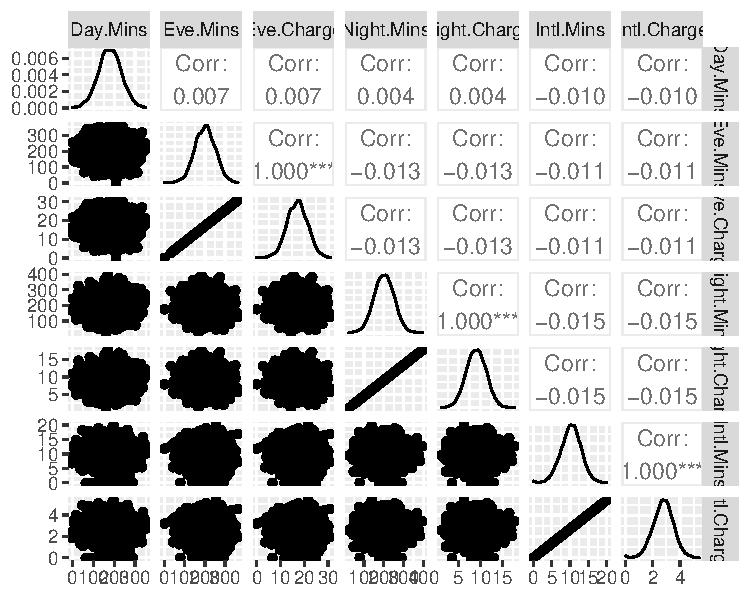
\includegraphics[width=\maxwidth]{figure/Pair_plot_for_continuous_variables-1} 

}



\end{knitrout}
Możemy zauważyć, że zmienne z przyrostkami `.Mins` oraz `.Charge` są ze sobą idealnie skorelowane. Odrzućmy zatem od razu dane z przyrostkiem `.Charge` dla ułatwienia dalszej analizy. Nie ma natomiast korelacji pomiędzy pozostałymi atrybutami.

\begin{knitrout}
\definecolor{shadecolor}{rgb}{0.969, 0.969, 0.969}\color{fgcolor}\begin{kframe}
\begin{alltt}
\hlstd{numerics} \hlkwb{<-} \hlkwd{subset}\hlstd{(numerics,} \hlkwc{select}\hlstd{=}\hlopt{-}\hlkwd{c}\hlstd{(Day.Charge, Eve.Charge, Night.Charge, Intl.Charge))}
\end{alltt}
\end{kframe}
\end{knitrout}

Wykonamy teraz wykresy zmiennych ilościowych, dzieląc klientów na dwie grupy:
\begin{itemize}
  \item tych, którzy zrezygnowali --- \verb|Churn. == TRUE |,
  \item tych, którzy pozostali lojalni --- \verb|Churn. == FALSE|.
\end{itemize}
\begin{knitrout}
\definecolor{shadecolor}{rgb}{0.969, 0.969, 0.969}\color{fgcolor}\begin{kframe}
\begin{alltt}
\hlstd{numerics} \hlkwb{<-} \hlkwd{data.frame}\hlstd{(numerics,} \hlkwc{Churn.} \hlstd{= df}\hlopt{$}\hlstd{Churn.)}
\end{alltt}
\end{kframe}
\end{knitrout}

Poniżej wykresy słupkowe dla danych jakościowych.
\begin{knitrout}
\definecolor{shadecolor}{rgb}{0.969, 0.969, 0.969}\color{fgcolor}\begin{kframe}
\begin{alltt}
\hlkwd{ggplot}\hlstd{(}\hlkwd{gather}\hlstd{(factors,} \hlstr{"key"}\hlstd{,} \hlstr{"value"}\hlstd{,} \hlopt{-}\hlstd{Churn.),} \hlkwd{aes}\hlstd{(value,} \hlkwc{fill}\hlstd{=Churn.))} \hlopt{+}
  \hlkwd{geom_bar}\hlstd{(}\hlkwc{position}\hlstd{=}\hlstr{"fill"}\hlstd{)} \hlopt{+}
  \hlkwd{facet_wrap}\hlstd{(}\hlopt{~}\hlstd{key,} \hlkwc{scales}\hlstd{=}\hlstr{'free'}\hlstd{)}
\end{alltt}
\end{kframe}

{\centering 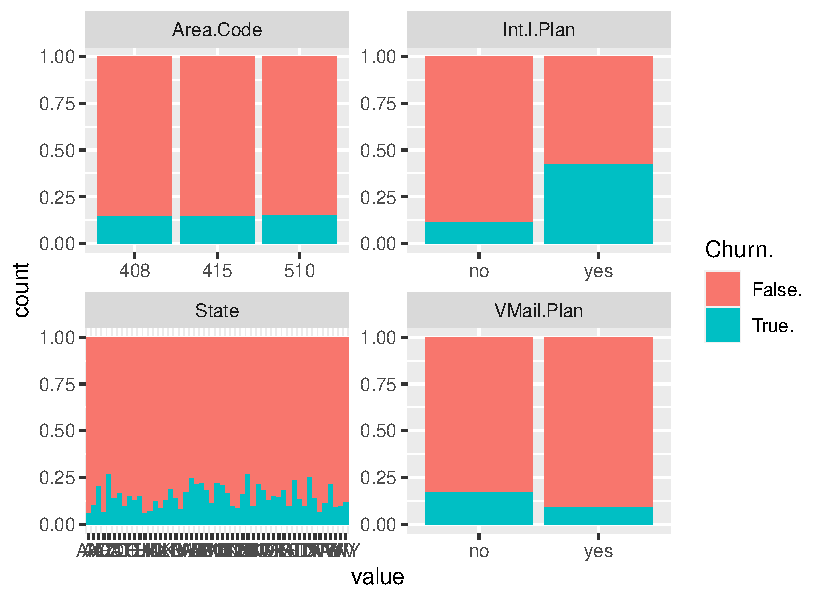
\includegraphics[width=\maxwidth]{figure/Bar_plots-1} 

}



\end{knitrout}

Możemy zauważyć, że osoby, które posiadały plan międzynarodowy, jak i te, które nie posiadały planu skrzyki głosowej częściej rezygnowały z usług. Zmienne \verb|Area.Code| i \verb|State| nie pokazują żadnych istotnych różnic pomiędzy tymi dwoma grupami.


Poniżej znajdują się wykresy empirycznych gęstości.
\begin{knitrout}
\definecolor{shadecolor}{rgb}{0.969, 0.969, 0.969}\color{fgcolor}\begin{kframe}
\begin{alltt}
\hlkwd{ggplot}\hlstd{(}\hlkwd{gather}\hlstd{(numerics,} \hlstr{"key"}\hlstd{,} \hlstr{"value"}\hlstd{,} \hlopt{-}\hlstd{Churn.),} \hlkwd{aes}\hlstd{(}\hlkwc{x}\hlstd{=value,} \hlkwc{color}\hlstd{=Churn.))} \hlopt{+}
  \hlkwd{geom_freqpoly}\hlstd{(}\hlkwd{aes}\hlstd{(}\hlkwc{y}\hlstd{=..density..),} \hlkwc{position}\hlstd{=}\hlstr{"identity"}\hlstd{)} \hlopt{+}
  \hlkwd{facet_wrap}\hlstd{(}\hlopt{~}\hlstd{key,} \hlkwc{scales}\hlstd{=}\hlstr{'free'}\hlstd{)}
\end{alltt}
\end{kframe}

{\centering 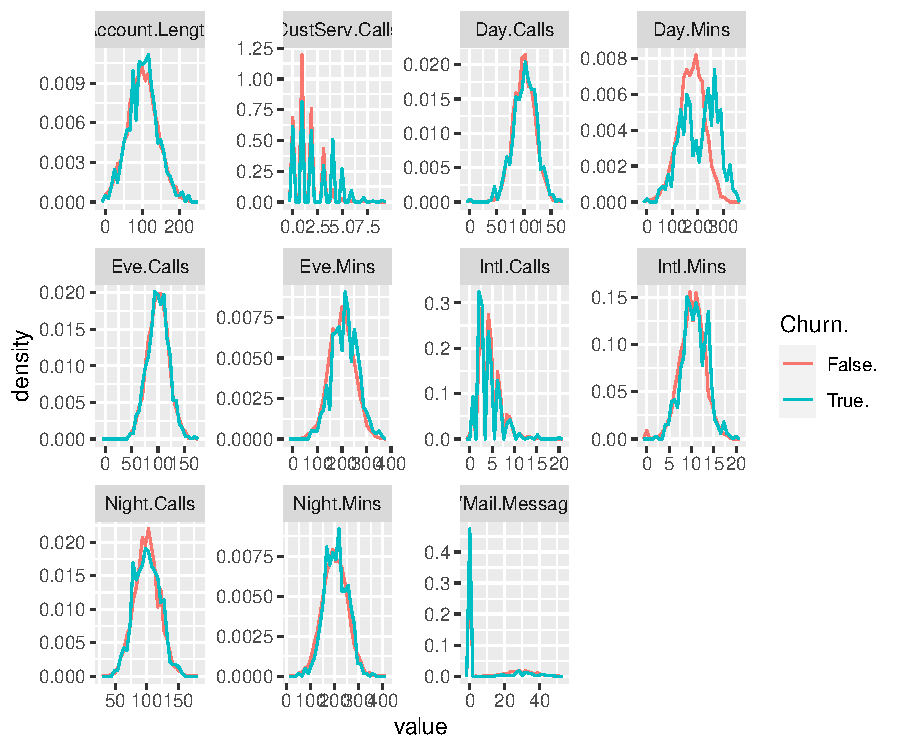
\includegraphics[width=\maxwidth]{figure/Densities-1} 

}



\end{knitrout}
Widoczne gołym okiem różnice są zauważalne w przypadku zmiennych: \verb|Day.Mins|, \verb|Customer.Service.Calls|, \verb|Eve.Calls|.

Poniżej generujemy wykresy pudełkowe. 
\begin{knitrout}
\definecolor{shadecolor}{rgb}{0.969, 0.969, 0.969}\color{fgcolor}\begin{kframe}
\begin{alltt}
\hlkwd{ggplot}\hlstd{(}\hlkwd{gather}\hlstd{(numerics,} \hlstr{"key"}\hlstd{,} \hlstr{"value"}\hlstd{,} \hlopt{-}\hlstd{Churn.),} \hlkwd{aes}\hlstd{(value,} \hlkwc{color}\hlstd{=Churn.))} \hlopt{+}
  \hlkwd{geom_boxplot}\hlstd{(}\hlkwd{aes}\hlstd{(}\hlkwc{x}\hlstd{=value))} \hlopt{+}
  \hlkwd{facet_wrap}\hlstd{(}\hlopt{~}\hlstd{key,} \hlkwc{scales}\hlstd{=}\hlstr{'free'}\hlstd{)}
\end{alltt}
\end{kframe}

{\centering 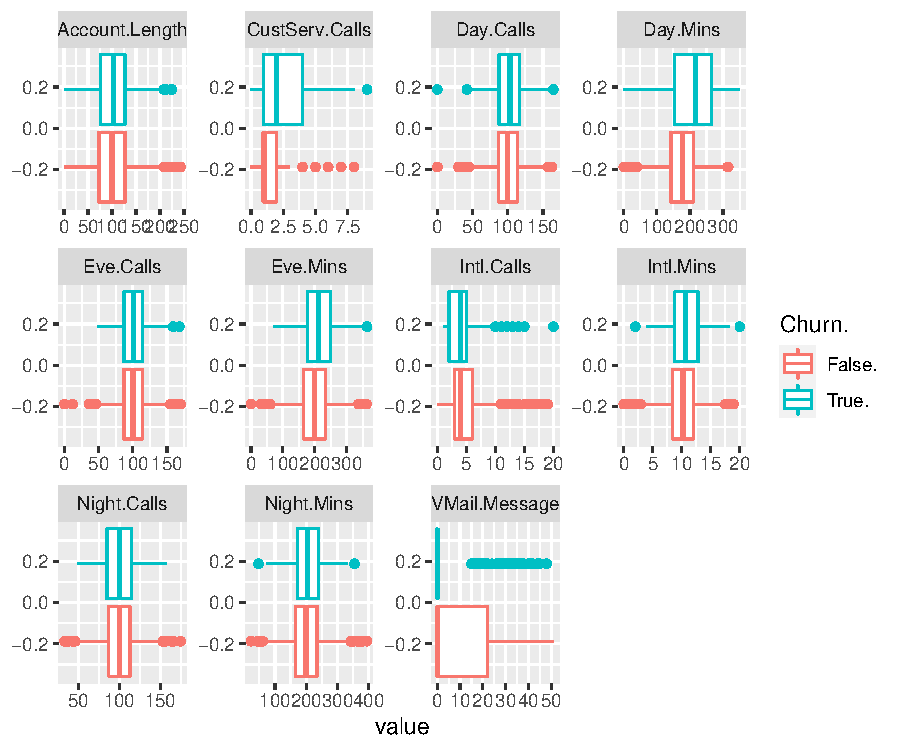
\includegraphics[width=\maxwidth]{figure/Boxplot-1} 

}



\end{knitrout}
Ponownie, duże różnice uwidaczniają się dla zmiennych: \verb|Day.Mins|, \verb|Customer.Service.Calls|, \verb|Eve.Calls|.

Stworzymy również wykresy empirycznych dystrybuant.
\begin{knitrout}
\definecolor{shadecolor}{rgb}{0.969, 0.969, 0.969}\color{fgcolor}\begin{kframe}
\begin{alltt}
\hlkwd{ggplot}\hlstd{(}\hlkwd{gather}\hlstd{(numerics,} \hlstr{"key"}\hlstd{,} \hlstr{"value"}\hlstd{,} \hlopt{-}\hlstd{Churn.),} \hlkwd{aes}\hlstd{(value,} \hlkwc{color}\hlstd{=Churn.))} \hlopt{+}
  \hlkwd{stat_ecdf}\hlstd{()} \hlopt{+}
  \hlkwd{facet_wrap}\hlstd{(}\hlopt{~}\hlstd{key,} \hlkwc{scales}\hlstd{=}\hlstr{'free'}\hlstd{)}
\end{alltt}
\end{kframe}

{\centering 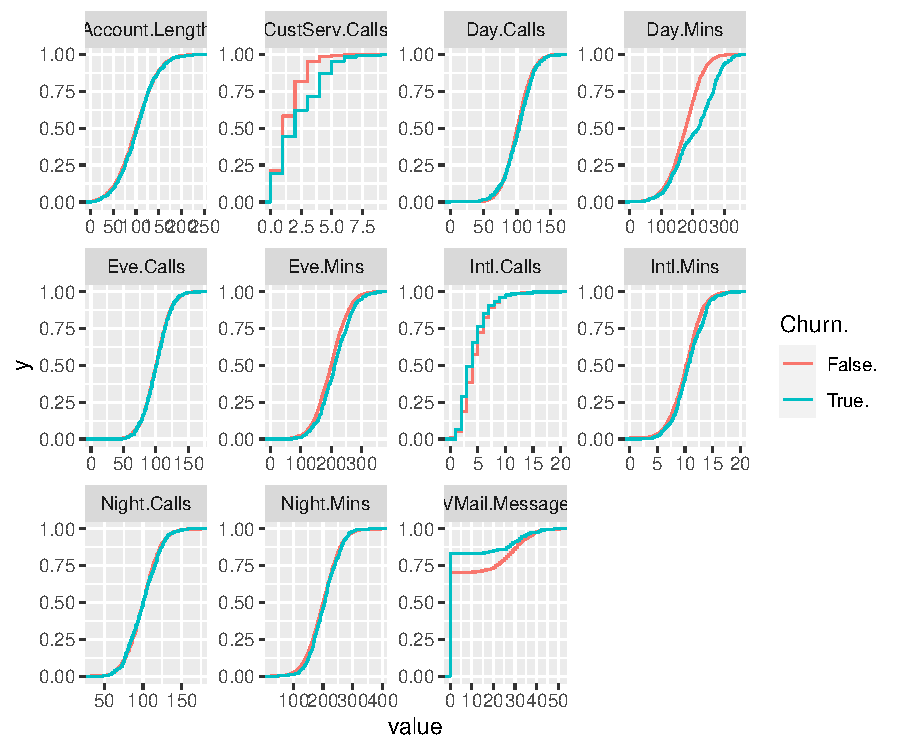
\includegraphics[width=\maxwidth]{figure/Ecdf-1} 

}



\end{knitrout}
Coś tam, coś tam \ldots

By wykryć, dla których zmiennych następuja najważniejsza różnica pomiędzy klientami lojalnymi, a tymi którzy zrezygnowali z usług, posłużymy się również testem Kołmogorova-Smirnova. Poniżej znajduje się funkcja, która wyznacza wyniki tego testu dla naszych zmiennych. 
\begin{knitrout}
\definecolor{shadecolor}{rgb}{0.969, 0.969, 0.969}\color{fgcolor}\begin{kframe}
\begin{alltt}
\hlstd{churn.kstest} \hlkwb{<-} \hlkwa{function}\hlstd{(}\hlkwc{feature}\hlstd{) \{}
  \hlstd{yes} \hlkwb{<-} \hlkwd{subset}\hlstd{(numerics,} \hlkwc{subset}\hlstd{=Churn.}\hlopt{==}\hlstr{"True."}\hlstd{)}
  \hlstd{no} \hlkwb{<-} \hlkwd{subset}\hlstd{(numerics,} \hlkwc{subset}\hlstd{=Churn.}\hlopt{==}\hlstr{"False."}\hlstd{)}
  \hlkwd{return}\hlstd{(}\hlkwd{c}\hlstd{(}\hlkwd{ks.test}\hlstd{(yes[[feature]], no[[feature]])[}\hlkwd{c}\hlstd{(}\hlstr{"statistic"}\hlstd{,} \hlstr{"p.value"}\hlstd{)]))}
\hlstd{\}}
\end{alltt}
\end{kframe}
\end{knitrout}

Tabela poniżej zbiera wyniki przeprowadzonych testów statystycznych.
\begin{table}[!h]

\caption{\label{tab:tabela_3}Wyniki testu Kolmogorova-Smirnova}
\centering
\resizebox{\linewidth}{!}{
\begin{tabular}[t]{l|r|r|r|r|r|r|r|r|r|r|r}
\hline
Zmienna & Account.Length & VMail.Message & Day.Mins & Day.Calls & Eve.Mins & Eve.Calls & Night.Mins & Night.Calls & Intl.Mins & Intl.Calls & CustServ.Calls\\
\hline
statistic & 0.0389430 & 0.1298071 & 0.3172082 & 0.0556326 & 0.1166198 & 0.0192285 & 0.0551378 & 0.0401351 & 0.1007606 & 0.1054201 & 0.2404511\\
\hline
pvalue & 0.5581609 & 0.0000018 & 0.0000000 & 0.1550801 & 0.0000264 & 0.9980118 & 0.1622501 & 0.5189055 & 0.0004560 & 0.0002062 & 0.0000000\\
\hline
\end{tabular}}
\end{table}


Możemy zauważyć, że testy na największe różnice (duża wartość zmiennej \verb|statistic|, mała zmiennej \verb|pvalue|) wskazują w przypadku zmiennych: CustServ.Calls, Day.Mins, Eve.Mins, 


Po dogłębnym przeanalizowaniu wykresów i wyników testów Kołmogorova-Smirnova, zauważmy, że istotne dla naszej analizy to następujące zmienne:
\begin{itemize}
  \item ilościowych:
    \begin{itemize}
    \item CustServ.Calls,
    \item Day.Mins,
    \item Eve.Mins;
    \end{itemize}
  \item jakościowych
    \begin{itemize}
    \item Int.l.Plan,
    \item VMail.Plan,
    \item Churn.
    \end{itemize}
\end{itemize}

\section{Analiza wybranych zmiennych}
Skupmy się jedynie na wybranych zmiennych:
\begin{knitrout}
\definecolor{shadecolor}{rgb}{0.969, 0.969, 0.969}\color{fgcolor}\begin{kframe}
\begin{alltt}
\hlstd{important} \hlkwb{<-} \hlkwd{subset}\hlstd{(df,} \hlkwc{select}\hlstd{=}\hlkwd{c}\hlstd{(CustServ.Calls, Day.Mins, Eve.Mins, Int.l.Plan,}
                                 \hlstd{VMail.Plan, VMail.Message, Churn.))}
\end{alltt}
\end{kframe}
\end{knitrout}

Wyznaczmy dla nich wskaźniki sumaryczne.

\begin{knitrout}
\definecolor{shadecolor}{rgb}{0.969, 0.969, 0.969}\color{fgcolor}\begin{kframe}
\begin{alltt}
\hlstd{my_summary} \hlkwb{<-} \hlkwa{function}\hlstd{(}\hlkwc{x}\hlstd{) \{}
  \hlstd{statistics} \hlkwb{<-} \hlkwd{c}\hlstd{(}\hlkwd{mean}\hlstd{(x),} \hlkwd{quantile}\hlstd{(x,} \hlnum{0.25}\hlstd{),} \hlkwd{median}\hlstd{(x),} \hlkwd{quantile}\hlstd{(x,} \hlnum{0.75}\hlstd{),}
                  \hlkwd{IQR}\hlstd{(x),} \hlkwd{min}\hlstd{(x),} \hlkwd{max}\hlstd{(x),} \hlkwd{var}\hlstd{(x),} \hlkwd{sd}\hlstd{(x),} \hlkwd{sd}\hlstd{(x)} \hlopt{/} \hlkwd{mean}\hlstd{(x),}
                  \hlkwd{kurtosis}\hlstd{(x),} \hlkwd{skewness}\hlstd{(x))}
  \hlkwd{names}\hlstd{(statistics)} \hlkwb{<-} \hlkwd{c}\hlstd{(}\hlstr{"Srednia"}\hlstd{,} \hlstr{"Q1"}\hlstd{,} \hlstr{"Mediana"}\hlstd{,} \hlstr{"Q3"}\hlstd{,} \hlstr{"IQR"}\hlstd{,} \hlstr{"Min"}\hlstd{,} \hlstr{"Max"}\hlstd{,}
                         \hlstr{"Wariancja"}\hlstd{,} \hlstr{"Odchylenie standardowe"}\hlstd{,} \hlstr{"Wspolczynnik zmiennosci"}\hlstd{,}
                         \hlstr{"Kurtoza"}\hlstd{,} \hlstr{"Skosnosc"}\hlstd{)}
  \hlkwd{return}\hlstd{(statistics)}
\hlstd{\}}
\end{alltt}
\end{kframe}
\end{knitrout}

\begin{table}[!h]

\caption{\label{tab:tabela_2}Wskazniki sumaryczne dla wybranych zmiennych}
\centering
\resizebox{\linewidth}{!}{
\begin{tabular}[t]{l|r|r|r|r|r|r|r|r|r|r|r|r}
\hline
  & Srednia & Q1 & Mediana & Q3 & IQR & Min & Max & Wariancja & Odchylenie standardowe & Wspolczynnik zmiennosci & Kurtoza & Skosnosc\\
\hline
CustServ.Calls & 1.562856 & 1.0 & 1.0 & 2.0 & 1.0 & 0 & 9.0 & 1.730517 & 1.315491 & 0.8417223 & 4.726519 & 1.0908683\\
\hline
Day.Mins & 179.775097 & 143.7 & 179.4 & 216.4 & 72.7 & 0 & 350.8 & 2966.696486 & 54.467389 & 0.3029752 & 2.978290 & -0.0290640\\
\hline
Eve.Mins & 200.980348 & 166.6 & 201.4 & 235.3 & 68.7 & 0 & 363.7 & 2571.894016 & 50.713844 & 0.2523324 & 3.023792 & -0.0238667\\
\hline
VMail.Message & 8.099010 & 0.0 & 0.0 & 20.0 & 20.0 & 0 & 51.0 & 187.371347 & 13.688365 & 1.6901282 & 2.947148 & 1.2642543\\
\hline
\end{tabular}}
\end{table}



Przedstawimy również wartości tych zmiennych na histogramach.

\begin{knitrout}
\definecolor{shadecolor}{rgb}{0.969, 0.969, 0.969}\color{fgcolor}\begin{kframe}
\begin{alltt}
\hlstd{subset} \hlkwb{=} \hlkwd{subset}\hlstd{(important,} \hlkwc{select}\hlstd{=}\hlopt{-}\hlkwd{c}\hlstd{(Churn., Int.l.Plan, VMail.Plan))}
\hlkwd{ggplot}\hlstd{(}\hlkwd{gather}\hlstd{(subset,} \hlstr{'key'}\hlstd{,} \hlstr{'value'}\hlstd{),} \hlkwd{aes}\hlstd{(}\hlkwc{x}\hlstd{=value))} \hlopt{+}
  \hlkwd{geom_histogram}\hlstd{(}\hlkwd{aes}\hlstd{(}\hlkwc{y}\hlstd{=..density..),} \hlkwc{position}\hlstd{=}\hlstr{"identity"}\hlstd{,} \hlkwc{color}\hlstd{=}\hlstr{"orange"}\hlstd{)} \hlopt{+}
  \hlkwd{facet_wrap}\hlstd{(}\hlopt{~}\hlstd{key,} \hlkwc{scales}\hlstd{=}\hlstr{'free'}\hlstd{)}
\end{alltt}
\end{kframe}

{\centering 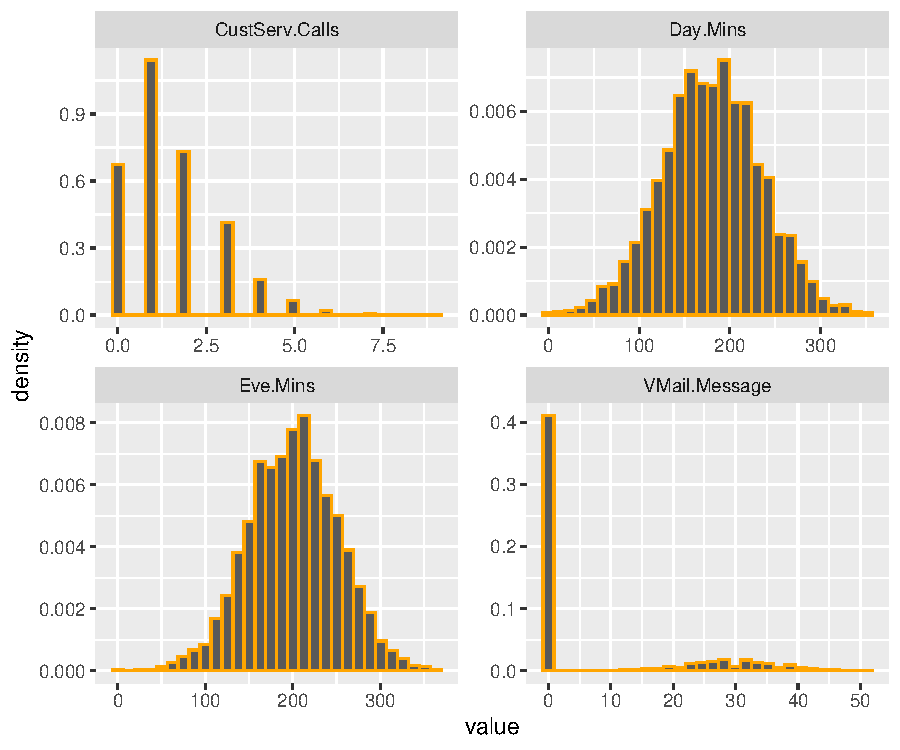
\includegraphics[width=\maxwidth]{figure/histograms-1} 

}



\end{knitrout}


\verb|Day.Mins| i \verb|Eve.Mins| mają rozkład symetryczny, natomiast pozostałe \verb|CustServ.Calls| i \verb|VMail.Message| mają rozkład prawostronnie skośny. Dodatkowo, te dwie zmiene charakteryzują się one dużą zmiennością.\newline
\vspace{0.3cm}
Teraz przyjrzyjmy się bliżej wybranym zmiennym jakościowym.

\begin{knitrout}
\definecolor{shadecolor}{rgb}{0.969, 0.969, 0.969}\color{fgcolor}\begin{table}[!h]
\centering
\begin{tabular}[t]{l|r}
\hline
Churn & Count\\
\hline
False. & 2850\\
\hline
True. & 483\\
\hline
\end{tabular}
\end{table}

\begin{table}[!h]
\centering
\begin{tabular}[t]{l|r}
\hline
Int.l.Plan & Count\\
\hline
no & 3010\\
\hline
yes & 323\\
\hline
\end{tabular}
\end{table}

\begin{table}[!h]
\centering
\begin{tabular}[t]{l|r}
\hline
VMail.Plan & Count\\
\hline
no & 2411\\
\hline
yes & 922\\
\hline
\end{tabular}
\end{table}


\end{knitrout}

Stworzymy dla tych zmiennych wykresy słupkowe.
\begin{knitrout}
\definecolor{shadecolor}{rgb}{0.969, 0.969, 0.969}\color{fgcolor}\begin{kframe}
\begin{alltt}
\hlkwd{ggplot}\hlstd{(}\hlkwd{gather}\hlstd{(important,} \hlstr{"key"}\hlstd{,} \hlstr{"value"}\hlstd{,} \hlopt{-}\hlkwd{c}\hlstd{(CustServ.Calls, Day.Mins, Eve.Mins, VMail.Message)),} \hlkwd{aes}\hlstd{(value))} \hlopt{+}
  \hlkwd{geom_bar}\hlstd{(}\hlkwc{position}\hlstd{=}\hlstr{"dodge"}\hlstd{,} \hlkwc{color}\hlstd{=}\hlstr{'orange'}\hlstd{)} \hlopt{+}
  \hlkwd{facet_wrap}\hlstd{(}\hlopt{~}\hlstd{key,} \hlkwc{scales}\hlstd{=}\hlstr{'free'}\hlstd{)}
\end{alltt}
\end{kframe}

{\centering 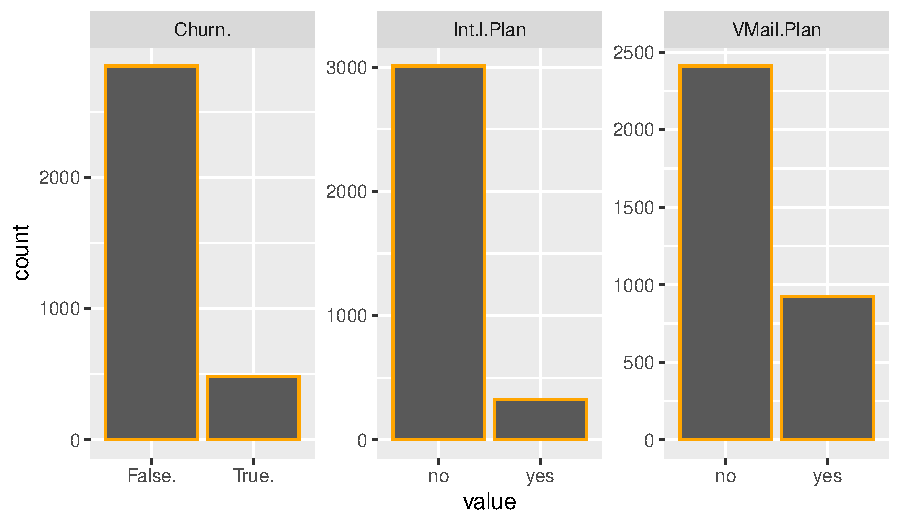
\includegraphics[width=\maxwidth]{figure/slupkowe_dla_wybranych-1} 

}



\end{knitrout}
Łatwo stwierdzić, że większośc klientów była lojalna ( $\approx 86$\%), nie miała wykupionego planu międzynarodowego ($\approx 90$ \%) oraz nie miało dostępu do planu poczty głosowej ($\approx 72$\%).  

\subsection{Analiza wybranych zmiennych z podziałem na grupy}

Poniższe tabele zawierają informacje o wartościach wskaźników sumarycznych dla zmiennych ilosciowych, tym razem uwzględniają one podział klientów na grupy.
\begin{knitrout}
\definecolor{shadecolor}{rgb}{0.969, 0.969, 0.969}\color{fgcolor}\begin{table}[!h]

\caption{\label{tab:sumaryczne dla grup}Day.Mins}
\centering
\resizebox{\linewidth}{!}{
\begin{tabular}[t]{l|r|r|r|r|r|r|r|r|r|r|r|r}
\hline
  & Srednia & Q1 & Mediana & Q3 & IQR & Min & Max & Wariancja & Odchylenie standardowe & Wspolczynnik zmiennosci & Kurtoza & Skosnosc\\
\hline
False. & 175.18 & 142.83 & 177.2 & 210.30 & 67.47 & 0 & 315.6 & 2518.2 & 50.18 & 0.29 & 2.99 & -0.23\\
\hline
True. & 206.91 & 153.25 & 217.6 & 265.95 & 112.70 & 0 & 350.8 & 4760.7 & 69.00 & 0.33 & 2.19 & -0.20\\
\hline
\end{tabular}}
\end{table}

\begin{table}[!h]

\caption{\label{tab:sumaryczne dla grup}Eve.Mins}
\centering
\resizebox{\linewidth}{!}{
\begin{tabular}[t]{l|r|r|r|r|r|r|r|r|r|r|r|r}
\hline
  & Srednia & Q1 & Mediana & Q3 & IQR & Min & Max & Wariancja & Odchylenie standardowe & Wspolczynnik zmiennosci & Kurtoza & Skosnosc\\
\hline
False. & 199.04 & 164.5 & 199.6 & 233.20 & 68.70 & 0.0 & 361.8 & 2529.30 & 50.29 & 0.25 & 3.03 & -0.04\\
\hline
True. & 212.41 & 177.1 & 211.3 & 249.45 & 72.35 & 70.9 & 363.7 & 2675.88 & 51.73 & 0.24 & 2.90 & 0.03\\
\hline
\end{tabular}}
\end{table}

\begin{table}[!h]

\caption{\label{tab:sumaryczne dla grup}CustServ.Calls}
\centering
\resizebox{\linewidth}{!}{
\begin{tabular}[t]{l|r|r|r|r|r|r|r|r|r|r|r|r}
\hline
  & Srednia & Q1 & Mediana & Q3 & IQR & Min & Max & Wariancja & Odchylenie standardowe & Wspolczynnik zmiennosci & Kurtoza & Skosnosc\\
\hline
False. & 1.45 & 1 & 1 & 2 & 1 & 0 & 8 & 1.35 & 1.16 & 0.80 & 4.21 & 0.89\\
\hline
True. & 2.23 & 1 & 2 & 4 & 3 & 0 & 9 & 3.43 & 1.85 & 0.83 & 2.89 & 0.70\\
\hline
\end{tabular}}
\end{table}

\begin{table}[!h]

\caption{\label{tab:sumaryczne dla grup}VMail.Message}
\centering
\resizebox{\linewidth}{!}{
\begin{tabular}[t]{l|r|r|r|r|r|r|r|r|r|r|r|r}
\hline
  & Srednia & Q1 & Mediana & Q3 & IQR & Min & Max & Wariancja & Odchylenie standardowe & Wspolczynnik zmiennosci & Kurtoza & Skosnosc\\
\hline
False. & 8.60 & 0 & 0 & 22 & 22 & 0 & 51 & 193.58 & 13.91 & 1.62 & 2.71 & 1.17\\
\hline
True. & 5.12 & 0 & 0 & 0 & 0 & 0 & 48 & 140.66 & 11.86 & 2.32 & 5.52 & 2.03\\
\hline
\end{tabular}}
\end{table}


\end{knitrout}

Podobnie jak powyżej, przedstawimy wartości zmiennych, korzystając z histogramów. Tym razem uwzględniamy podział na grupy.

\begin{knitrout}
\definecolor{shadecolor}{rgb}{0.969, 0.969, 0.969}\color{fgcolor}\begin{kframe}
\begin{alltt}
\hlstd{subset} \hlkwb{=} \hlkwd{subset}\hlstd{(important,} \hlkwc{select}\hlstd{=}\hlopt{-}\hlkwd{c}\hlstd{(Int.l.Plan, VMail.Plan))}
\hlkwd{ggplot}\hlstd{(}\hlkwd{gather}\hlstd{(subset,} \hlstr{'key'}\hlstd{,} \hlstr{'value'}\hlstd{,} \hlopt{-}\hlstd{Churn.),} \hlkwd{aes}\hlstd{(}\hlkwc{x}\hlstd{=value,} \hlkwc{color}\hlstd{=Churn.))} \hlopt{+}
  \hlkwd{geom_histogram}\hlstd{(}\hlkwd{aes}\hlstd{(}\hlkwc{y}\hlstd{=..density..),} \hlkwc{position}\hlstd{=}\hlstr{"identity"}\hlstd{)} \hlopt{+}
  \hlkwd{facet_wrap}\hlstd{(}\hlopt{~}\hlstd{key,} \hlkwc{scales}\hlstd{=}\hlstr{'free'}\hlstd{)}
\end{alltt}
\end{kframe}

{\centering 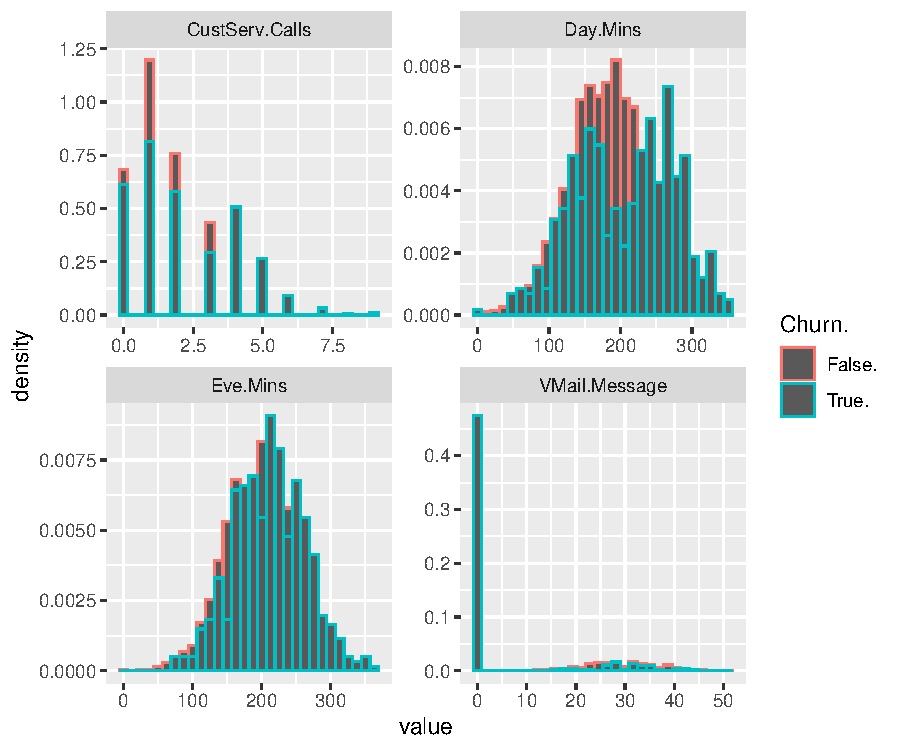
\includegraphics[width=\maxwidth]{figure/histogramy_dla_grup-1} 

}



\end{knitrout}

Zauważamy, że 

\vspace{0.3cm}

Przyjrzymy się teraz zmiennym jakościowym po podziale na grupy.

\begin{knitrout}
\definecolor{shadecolor}{rgb}{0.969, 0.969, 0.969}\color{fgcolor}\begin{table}[!h]

\caption{\label{tab:ilosciowe dla grup}Int.l.Plan}
\centering
\begin{tabular}[t]{l|r|r}
\hline
  & False. & True.\\
\hline
no & 0.89 & 0.11\\
\hline
yes & 0.58 & 0.42\\
\hline
\end{tabular}
\end{table}

\begin{table}[!h]

\caption{\label{tab:ilosciowe dla grup}VMail.Plan}
\centering
\begin{tabular}[t]{l|r|r}
\hline
  & False. & True.\\
\hline
no & 0.83 & 0.17\\
\hline
yes & 0.91 & 0.09\\
\hline
\end{tabular}
\end{table}


\end{knitrout}

Wykonamy także wykresy rozrzutu, przedstawiające zależności między zmiennymi ilościowymi.

\begin{knitrout}
\definecolor{shadecolor}{rgb}{0.969, 0.969, 0.969}\color{fgcolor}\begin{kframe}
\begin{alltt}
\hlstd{subset} \hlkwb{=} \hlkwd{subset}\hlstd{(important,} \hlkwc{select}\hlstd{=}\hlopt{-}\hlkwd{c}\hlstd{(Int.l.Plan, VMail.Plan))}
\hlstd{subset} \hlopt \hlkwd{ggpairs}\hlstd{(.,}
\hlkwc{mapping} \hlstd{= ggplot2}\hlopt{::}\hlkwd{aes}\hlstd{(}\hlkwc{color}\hlstd{=Churn.),}
\hlkwc{columns}\hlstd{=}\hlnum{1}\hlopt{:}\hlnum{4}\hlstd{,}
\hlkwc{lower}\hlstd{=}\hlkwd{list}\hlstd{(}\hlkwc{continuous}\hlstd{=}\hlkwd{wrap}\hlstd{(}\hlstr{"points"}\hlstd{,} \hlkwc{alpha}\hlstd{=}\hlnum{.4}\hlstd{,} \hlkwc{size}\hlstd{=}\hlnum{.01}\hlstd{)),}
\hlkwc{upper}\hlstd{=}\hlkwd{list}\hlstd{(}\hlkwc{continuous}\hlstd{=}\hlstr{"blank"}\hlstd{),}
\hlkwc{diag}\hlstd{=}\hlkwd{list}\hlstd{(}\hlkwc{continuous}\hlstd{=}\hlstr{"blank"}\hlstd{))}
\end{alltt}
\end{kframe}

{\centering 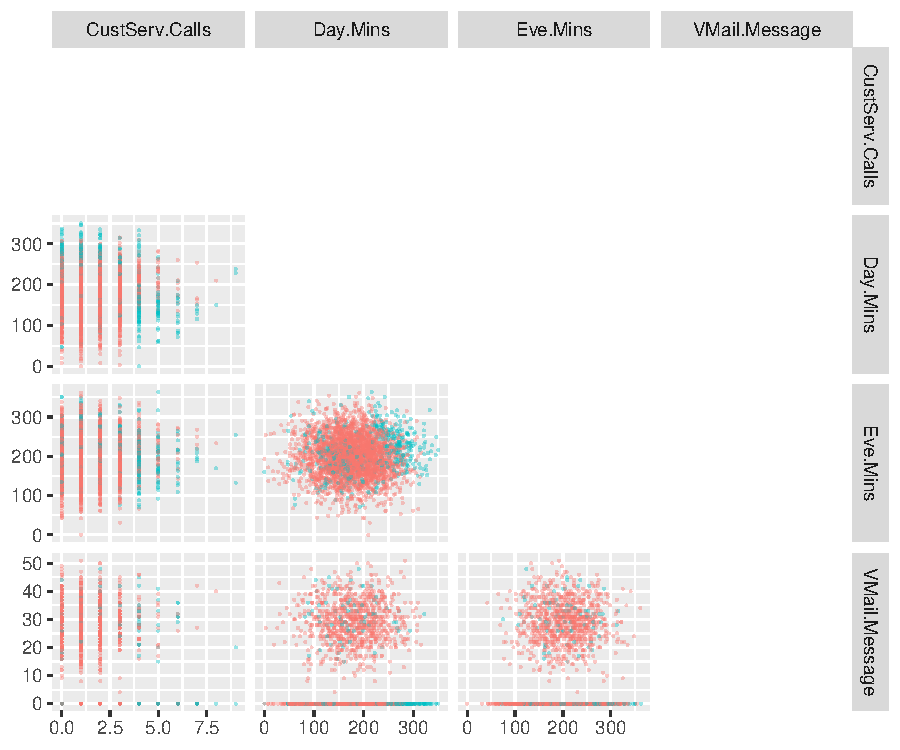
\includegraphics[width=\maxwidth]{figure/scatterplot-1} 

}



\end{knitrout}


\section{Podsumowanie}
Najważniesze wnioski z naszej analizy to:
\begin{itemize}
  \item jakiś wniosek
\end{itemize}

\end{document}
